%Template pembuatan proposal skripsi.
\documentclass{jtetiproposalskripsi}

%-----------------------------------------------------------------
%Disini awal masukan untuk data proposal skripsi
%-----------------------------------------------------------------
\titleind{PENGONTROL SUHU BERBASIS
MIKROKONTROLER 

}

\fullname{Rizaldi Rahman Waskito}

\idnum{1110651133}

\approvaldate{15 Januari 2015}

\degree{Sarjana Komputer}

\yearsubmit{2015}

\program{Teknik Informatika}

\headprogram{Triawan Adi Cahyanto M.Kom.}

\dept{Teknik}

\firstsupervisor{Ari Eko Wardoyo, S.T., M.Kom}
\firstnip{1975 0214 2005 01 1 001}

\secondsupervisor{}
\secondnip{}


%-----------------------------------------------------------------
%Disini akhir masukan untuk data proposal skripsi
%-----------------------------------------------------------------

\begin{document}

\cover

\approvalpage

%-----------------------------------------------------------------
%Disini akhir masukan untuk muka skripsi
%-----------------------------------------------------------------

%-----------------------------------------------------------------
%Disini awal masukan Intisari
%-----------------------------------------------------------------
\begin{abstractind}
Dalam merancang sistem pengukuran suhu ruang berbasisikan mikrokontroler AT89C52 ini timbul beberapa masalah, antara lain mengenai bagaimana rancangan perangkat kerasnya, dan mengenai perancangan program yang berfungsi untuk menjalankan rangkaian sistem tersebut. Tujuan dari perancangan sistem ini adalah agar dapat membantu manusia mengetahui perubahan suhu suatu ruang. Pada intinya rangkaian sistem ini dirancang untuk mengubah perubahan suhu yang terjadi pada sebuah sensor menjadi nilai digital dan menampilkannya pada komputer dengan menggunakan ADC dan mikrokontroler dimana komunikasi antara alat dengan komputer dengan serial.. Dengan pengujian pada sistem yang telah dilakukan didapatkan bahwa sistem ini mampu menyimpan data pada memori alat sebanyak 192 alamat data. Ketika alamat yang diperuntukkan untuk menyimpan data telah penuh maka alat akan berhenti menyimpan data namun tetap menampilkan perubahan suhu yang terdeteksi oleh sensor suhu. Selain itu data pengukuran dapat disimpan pada komputer sebagai penyimpan data permanen. Data yang telah disimpan dapat dipanggil kembali dan ditampilkan dalam bentuk grafik. Alat ini mampu mengukur suhu secara presisi mulai dari 26C - 100C, dengan toleransi kesalahan +0C - 2C. Sehingga dapat disimpulkan bahwa alat berfungsi dengan baik dan keluarannya sesuai dengan apa yang diharapkan dan sesuai dengan tujuan awal penelitian dan perancangan sistem ini.





\bigskip
\textbf{Kata kunci} : \emph{Sensor Suhu}, \emph{, Perubahan Suhu ke Besaran Digital}, \emph{Mikrokontroler AT89C52}, \emph{ADC0804}, \emph{Komunikasi Serial}
\end{abstractind}
%-----------------------------------------------------------------
%Disini akhir masukan Intisari
%-----------------------------------------------------------------

\tableofcontents
\addcontentsline{toc}{chapter}{DAFTAR ISI}
\selectlanguage{bahasa}\clearpage\pagenumbering{arabic}\setcounter{page}{1}

%-----------------------------------------------------------------
%Disini awal masukan untuk Bab
%-----------------------------------------------------------------
\chapter{LATAR BELAKANG}

\section{Latar Belakang Masalah}
Pada masa sekarang ini bidang elektronika mengalami kemajuan yang sangat pesat dan tidak terlepas pada bidang komputerisasi. Komputer saat ini telah menjadi alat bantu utama bagi manusia dan digunakan bukan hanya untuk menyelesaikan permasalahan di tempat kerja, membuat program atau bermain game, tetapi dapat digunakan untuk mengontrol alat melalui berbagai port yang tersedia dan dikenal dengan istilah interfacing komputer (hubungan antar muka komputer). Dan ini sangat membuat penulis tertarik untuk membuat sebuah alat yang dikontrol oleh komputer. 



Dengan adanya teknologi yang terus berkembang saat ini, maka akan semakin mudah untuk mengetahui apakah tanda-tanda aktifitas itu akan berprospek menjadi bencana alam ataukah dapat dimanfaatkan. 



Salah satu teknologi terapan itu adalah alat yang berfungsi untuk mengukur suhu panas bumi. Namun peralatan yang ada sekarang masih sederhana sehingga memerlukan pengembangan teknologi yang lebih efektif sehingga teknisi tidak harus selalu siap di lapangan untuk mencatat setiap perubahan suhu dengan rentang waktu tertentu sesuai yang diperlukan pada saat pengambilan sample suhu untuk kemudian diteliti lebih lanjut supaya dapat ditindaklanjuti baik dampak positif maupun negatifnya.



Lalu timbul ide penulis untuk membuat sistem pengukuran suhu ruangan, yang dibangun sebagai suatu sistem  yang mampu mengukur perubahan suhu dan menyimpan data pengukuran itu pada memori internal alat sebagai penyimpan data sementara untuk dipindahkan ke komputer sebagai penyimpan data permanen, sehingga akan lebih mengefektifkan waktu dan biaya operasional karena alat ini mempunyai fasilitas yang lebih lengkap dan menunjang.



\section{Perumusan dan Pembatasan Masalah}

Dalam merancang sistem perangkat keras pengukuran suhu timbul beberapa masalah. Masalah-masalah itu antara lain mengenai bagaimana rancangan perangkat kerasnya. Masalah berikutnya adalah mengenai perancangan program yang berfungsi untuk menjalankan rangkaian.



\section{Tujuan}

Penelitian ini bertujuan untuk membuat suatu rancang bangun perangkat keras yang dapat mendeteksi suhu suatu ruangan yang lebih akurat, serta program pendukung rangkaian perangkat kerasnya.



\section{Manfaat}

Memberikan informasi kepada pembaca tentang pembuatan dan pemanfaatan aplikasi mikrokontroler pada sistem minimum. Dapat digunakan sebagai pengukur suhu pada gunungan sampah pada tempat pembuangan akhir, dan atau pengukur suhu pada proses fermentasi jerami untuk penanaman jamur. Digunakan sebagai bahan referensi atau kajian untuk pengembangan selanjutnya bagi peneliti lain. Memberikan suatu alternatif teknologi terapan yang dapat lebih mengefektifkan waktu dan biaya operasional serta validitas data yang dibutuhkan ketika digunakan pada kegiatan lapangan.






%-------------------------------------------------------------------------------
\chapter{DASAR TEORI}                

\section{Konsep Suhu [1,2]}

Suhu merupakan derajat panas dari suatu benda. Dari sentuhan telapak tangan, kita dapat menyusun urutan benda-benda berdasarkan derajat panasnya dari benda A, B, dan C, kita dapat memutuskan bahwa B lebih panas dari A, C lebih panas dari B. Kita dapat menyatakan bahwa suhu yang paling tinggi adalah C, dan yang paling rendah adalah A. Jadi, konsep suhu berasal dari perasaan kita.


	
Kita dapat merasakan panas atau dingin suatu benda dengan menyentuhnya. Akan tetapi, apakah perasaan kita dapat menyatakan suhu benda dengan tepat ? Percobaan sederhana ini pertama kali disarankan oleh John Locke pada tahun 1960. Mula-mula kita celupkan tangan kiri pada ember yang berisi air dingin dan tangan kanan pada ember yang berisi air hangat selama kira-kira 30 detik. Yang dimaksud air hangat di sini adalah air yang paling panas yang dapat ditahan oleh kulit tangan ita selama kira-kira 30 detik. Dengan cepat pindahkan kedua tangan kita ke dalam ember ketiga yang berisi air yang suhunya di antara air dingin dan hangat. Air terasa lebih sejuk untuk tangan kanan dan lebih hangat untuk tangan kiri.
	
	
	
Hasil percobaan diatas menunjukkan perasaan kita keliru menilai suhu. Selain itu, jangkauan perasaan kita adalah terbatas. Tangan kita tidak tahan menyentuh benda yang sangat panas atau sangat dingin. Oleh karena itu, diperlukan suatu alat yang dapat kita gunakan untuk mengukur suhu dan menyatakannya dengan suatu angka. Alat untuk mengukur suhu disebut termometer.
	
	
	
Suhu secara umum dapat diukur dalam tiga skala yang berbeda yaitu Celcius, Fahrenhait dan Kelvin. Skala Celcius mempunyai titik didih air 100OC dan titik beku air 0OC. Skala Fahrenhait mempunyai titik didih air 212OF dan titik beku air 32OF. Sedangkan untuk skala Kelvin didasari oleh skala Celcius. Untuk mengubah dari Celcius ke Kelvin dengan menambahkan 273O pada skala Celcius yang terukur.
	
	
	
Suhu dapat diukur dalam berbagai macam cara yang berbeda. Dalam hal ini pengukuran suhu secara garis besar dapat dibedakan menjadi dua macam yaitu pengukuran secara mekanik dan pengukuran secara elektrik. Pengukuran secara mekanik tergantung pada beberapa prinsip fisik bahwa gas, zat cair dan zat padat dapat berubah volumenya apabila benda tersebut dipanaskan. Penggunaan substansi zat yang tidak sama dapat merubah volume dalam perbedaan kuantitas zat tersebut. Sebagai contoh, air raksa mempunyai penambahan 0,01% per derajat Fahrenhait sedangkan alkohol di lain pihak mempunyai penambahan 0,07% per derajat Fahrenhait (0,1% per derajat Celcius). Yang termasuk dalam pengukuran mekanik antara lain termometer glass-steam, termometer bimetallic, termometer filled-system. Sedangkan pengukuran secara elektrik menggunakan energi listrik untuk mengontrol perubahan suhu secara analog maupun secara digital dan mempunyai prinsip yang hampir sama dengan secara mekanik. Pengukuran perubahan suhu tersebut dapat dideteksi dengan menggunakan beberapa sensor antara lain thermocouple, thermistor, RTD IC Op-Amp, IC LM 35 dan lain sebagainya.
	
	
	
Banyak sifat fisis yang dapat diukur berubah sewaktu suhu yang diterima oleh benda tersebut berubah kuantitasnya. Di antara sifat-sifat ini adalah volume sebuah cairan, panjang sebuah tongkat, hambatan listrik sebuah kawat, tekanan sebuah gas pada volume konstan, volume gas pada tekanan konstan dan warna sebuah kawat pijar (filament). Masing-masing sifat ini dapat digunakan dalam pembuatan sebuah alat ukur suhu (termometer). Skala suhu yang didapat yaitu dengan memilih sebuah zat dan sifat termometrik yang khas dari zat tersebut. Apabila dalam memilih zat termometrik sudah didapat dan sifat termometrik tersebut dinyatakan dengan X dalam pembuatan sebuah sklala termometer maka dapat dipilih sembarang fungsi linier dari sifat X sebagai temperatur T yang dimiliki oleh termometer yang sesuai, dan setiap sistem yang berada di dalam kesetimbangan termal dengan termometer akan didapatkan sebuah persamaan : T(x) = aX. Di mana a adalah konstanta yang harus dihitung dengan memilih bentuk linier dari T(x) konstanta a ditentukan dengan mengkalibrasi termometer tersebut untuk menentukan sebuah titik tetap standart. Titik tetap ini merupakan titik di mana es, air cair dan uap air berada dalam kesetimbangan dan dinamakan dengan titik tripel air (triple point of water).
	


\section{Sensor Suhu [3,4,5]}

Sebagai sensor suhu seri LM 35 adalah intergrated-circuit (IC) sensor suhu yang presisi, mempunyai tegangan keluaran yang linier terhadap temperatur celcius. LM 35 tidak memerlukan kalibrasi atau trimming eksternal, karena sudah tersedia ketelitian ±1/4 oC pada suhu kamar dan ±3/4 oC atas suatu penuh, dalam cakupan temperatur –55 oC sampai +150 oC.


Keistimewaan dari sensor ini antara lain adalah dapat dikalibrasi langsung dalam oC, Keluaran sensor akan naik sebesar 10mV setiap derajat celcius dengan rentang temperatur sebesar -55 sampai 150OC, beroperasi pada tegangan 4 sampai 30 volt, sesuai untuk aplikasi jarak jauh dan  harga relatif terjangkau.

Untuk selanjutnya pada alat ini akan terjadi penguatan. Dimana untuk penguatan tersebut menggunakan IC Op-Amp LM 358. LM 358 adalah Op-Amp yang beroperasi dengan sumber daya tunggal, memiliki input berbeda, dan tetap berada dalam mode linier dengan masukan tegangan common 0 VDC. IC ini mampu bekerja pada beragam variasi tegangan sumber daya.



LM358 merupakan IC Op-Amp atau penguat yang mempunyai beberapa keunggulan dibanding Op-Amp lain ketika diaplikasikan secara tunggal. Komponen ini mampu bekerja pada tegangan dari 3 Volt hingga 32 Volt. LM 358 mempunyai duah buah Op-Amp yang sudah terintegrasi di dalamnya.


\section{Prinsip Pengubah Suhu ke Besaran Digital}
Untuk mengubah suhu dari besaran yang analog ke besaran digital, terlebih dahulu dicari perubahan atau nilai 1oC sama dengan berapa volt.Setelah didapatkan nilai 1oC sama dengan berapa volt, kemudian hasil tegangan keluaran yang didapat dikuatkan dengan cara mengalikan tegangan keluaran dengan rumus 2.1. Dimana rumus 2.1. merupakan rumus penguatan tak membalik dari op amp.




Dari hasil perhitungan diatas, maka didapatkan tegangan keluaran setelah dikuatkan. Hasil perhitungan tegangan yang telah dikuatkan tersebut akan dijadikan sebagai tegangan masukan untuk ADC. Untuk perhitungan di ADC digunakanlah rumus 2.2. Setelah dimasukkan ke dalam rumus 2.2. maka didapatlah nilai pengubahan besaran suhu yang dari analog ke besaran digital. 

\section{Mikrokontroler AT89C52 }
Mikrokontroler merupakan komputer mikro yang memadukan  CPU, ROM, RWM, I/O seri, counter-timer, dan rangkaian detak dalam satu chip tunggal. Penggunaan pokok dari mikrokontroler adalah mengontrol kerja mesin atau sistem dengan menggunakan program yang disimpan pada ROM.




Penggunaan mikrokontroler dalam suatu sistem minimum lebih menguntungkan dibandingkan dengan mikroprosesor sebab  mikrokontroler tidak membutuhkan lagi memori dan I/O eksternal selama memori dan I/O internal dalam chip masih mencukupi.




AT89C52 didisain dengan logika setatis untuk operasi frekuensi down to zero dan mendukung dua perangkat lunak mode saving power yang dapat dipilih. Mode idle berarti menghentikan kerja CPU sementara membiarkan RAM, timer, port serial dan sistem interupsi untuk terus bekerja. Mode power down menyimpan isi dari RAM tetapi menon-aktifkan oscillator sampai di-reset kembali.

\section{Perangkat Keras Mikrokontroler AT89C52 }
Mikrokontroler jenis AT89C52 adalah mikrokontoler dengan 8Kbyte Programmable and Eraseable Read Only Memory (PEROM) yang mempunyai fitur sebagai berikut :
1.Compatible dengan produk MCS-51

2.Mempunyai sitem memory flash 8 KByte yang dapat diprogram ulang sampai 1000 kali tulis / siklus hapus


3.Dapat  beroperasi statis secara penuh pada frekuensi 0 Hz sampai 24 MHz

4.Mempunyai  3 tingkat pengunci program memori

5.Mempunyai 256 X 8 bit RAM Internal

6.Memiliki 32 jalur I/O yang dapat diprogram

7.Memiliki 3 buah timer / counter 16 Bit

8.Memiliki saluran / kanal serial yang dapat diprogram

9.Memiliki 8 Sumber Interupsi

10.Low Power Middle and Power modes

\section{. Konfigurasi Kaki-Kaki Mikrokontroler AT89C52 }
Susunan kaki-kaki pada Mikrokontroler AT89C52 dapat diperhatikan pada gambar seperti dibawah ini:

\begin{figure}[ht!]
  \centering
    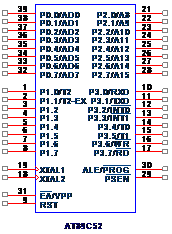
\includegraphics{gambar/1}
    \caption{ Konfigurasi Kaki Mikrokontroler AT89C52 }
    \label{kripto}
\end{figure}

Penjelasan dari masing-masing kaki mikrokontroler AT89C52 adalah sebagai berikut:
-	Vcc

	Memberikan tegangan supplay.
	
-	GND

Sebagai ground terhadap sumber.

-	Port 0

Port 0 dapat berfungsi sebagai I/O biasa, low order multiplex address/data, atau menerima kode byte pada saat Flash Programming. Port 0 merupakan port I/O 8 bit dua arah. Pada saat sebagai port keluaran masing – masing pinnya dapat menangani 8 input TTL. Saat 1 detik dimasukkan ke port 0, maka port ini akan berfungsi sebagai input dengan impedansi tinggi. Pada saat sebagai low order multiplex address/data port ini akan mempunyai internal pull up dan pada saat Flash Programming diperlukan external pull up terutama pada saat verifikasi program.

-	Port 1

Port 1 dapat berfungsi sebagai I/O biasa, low order multiplex address/data, atau menerima kode byte pada saat pemrograman Flash dan verifikasi. Saat logika 1 dituliskan pada pin port 1, maka akan ditarik naik oleh internal pull up dan dapat berfungsi sebagai masukan. Pin 0 dan 1 pada port 1 dapat berfungsi sebagai timer/counter 2 masukan external count (P1.0/T2) dan timer/counter 2 trigger (P1.1/T2EX).  Port 1 merupakan port I/O 8 bit dua arah  dengan internal pull up. Pada saat sebagai port keluaran masing – masing masukannya dapat menangani 4 input TTL.

-	Port 2

Merupakan port I/O 8 bit dua arah dengan internal pull up. Pada saat sebagai port keluaran masing–masing pinnya dapat menangani 4 input TTL. Saat logika 1 dimasukkan pada pin dari port 2, maka akan di pull up oleh internal pull up dan dapat berfungsi sebagai masukan. Port 2 mengeluarkan high-order address byte selama mengambil dari eksternal program memori dan selama mengakses eksternal data memori yang menggunakan 16-bit alamat (MOVX@DPTR). Selama mengakses eksternal data memori yang menggunakan 8-bit alamat (MOVX@RI), port 2 mengeluarkan isi dari P2 SFR. Port 2 juga menerima kode byte saat pemrograman flash dan verifikasi.

-	Port 3

Merupakan port I/O 8 bit dua arah dengan internal pull up. Pada saat sebagai port keluaran masing – masing pinnya dapat menangani 4 input TTL. Port 3 juga menerima kode byte saat pemrograman flash dan verifikasi. Selain itu, port 3 juga dapat bekerja sebagai fungsi – fungsi khusus pada AT89C51, yaitu :



-	RST

Masukan Reset tinggi pada pin selama 2 siklus mesin ketika osilator menjalankan reset peralatan.


-	ALE / PROG

Address Latch Enable mengeluarkan pulsa untuk byte rendah pada alamat selama mengakses memori eksternal. Pin ini juga sebagai input pulsa program ( PROG ) selama memprogram flash.


-	PSEN

PSEN (Program Store Enable ) adalah read strobe untuk memori program eksternal. Ketika AT89C52 mengeksekusi kode dari memori program eksternal. PSEN diaktifkan 2 X tiap siklus mesin.


-	EA / Vpp

Eksternal Access Enable harus dihubungkan dengan ground agar peralatan dapat mengambil kode dari memori program eksternal dimulai pada lokasi 0000H sampai alamat FFFFH, catatan jika lock bit 1 diprogram, EA akan menjadi pengunci internal pada reset. EA harus dipasang ke VCC untuk mengeksekusi program internal.


-	XTAL 1

Masukan untuk penguat osilator pembalik dan masukan untuk rangkaian operasi detak internal.


-XTAL 2

Keluaran dari penguat osilator pembalik.

\section{Konsep Transfer Data Serial }

Untuk jarak jauh biasanya digunakan transfer data secara serial, yaitu data dikirim melalui satu kabel atau satu bit pada satu waktu, dimana bit-bit yang ada pada suatu byte data harus menunggu giliran untuk dipindahkan. Berdasarkan arahnya, komunikasi data serial dibagi menjadi :

1.	Simplex

Pada sistem ini, komunikasi terjadi satu arah saja, dari pengirim (A) ke penerima (B). Penerima (B) tidak dapat mengirim ke pengirim (A).

2.	Half Duplex

Merupakan komunikasi 2 arah, misalnya antara A dan B. Pada saat A mengirim data, B hanya dapat menerima saja. Demikian juga sebaliknya, pada saat B mengirim data, A juga hanya dapat menerima. 

3.	Full Duplex

Contoh umum full duplex adalah komunikasi melalui jaringan telpon. Pada saat yang sama, kedua pihak yang berkomunikasi dapat mengirim atau menerima data.

%-------------------------------------------------------------------------------
\chapter{RANCANGAN SISTEM PENGUKURAN SUHU RUANG
BERBASISKAN MIKROKONTROLER AT89C52  
}

\section{Analisis Rangkaian Secara Diagram Balok}
Pada blok pertama terdapat blok masukan. Dimana pada blok ini terdapat sensor suhu yang menggunakan IC LM35 sebagai sensornya. Sensor ini sangat berpengaruh sekali, karena apabila diletakkan pada suatu ruangan, maka sensor akan langsung bekerja mengukur suhu yang ada diruangan tersebut. Hasil dari pengukuran suhu yang di deteksi oleh LM35 adalah berupa tegangan. Keluaran dari LM 35 akan menjadi masukan pada IC LM 358 dan akan di teruskan ke ADC 0804.




IC LM 358 digunakan sebagai penguat. Rangkaian penguat ini diperlukan karena kenaikan sebesar 10 mV setiap derajat celcius tidak dapat langsung dihubungkan ke ADC 0804 karena berada di bawah toleransi ketelitian. Tingkat kenaikan tegangan yang lebih kecil dari toleransi ketelitian ADC 0804 akan menyebabkan kesalahan dalam pengukuran. Untuk menghindari kesalahan tersebut maka diperlukan rangkaian penguatan dengan menggunakan LM 358 serta dengan konfigurasi penguatan tak membalik. Resistor R 10kΩ dan potensiometer 50kΩ dapat digunakan untuk mengatur agar keluaran dari LM 35 menjadi lima kali lebih besar. Sehingga keluarannya dapat menghasilkan tegangan




sebesar 50mV untuk setiap derajat celcius.
LM 358 pada rangkaian penguat ini menggunakan sumber tegangan sebesar 12 volt sehingga dioda zener dan resistor R1 digunakan pada keluaran penguat ini untuk menjaga agar batas maksimum tegangan hanya mencapai 5 volt saja dan melindungi ADC 0804 dari tegangan berlebih. Keluaran dari penguat ini selanjutnya akan masuk ke ADC 0804 pada kaki 6 (masukan analog).




ADC0804 mempunyai sebuah saluran masukan analog. Pemilihan ini dikarenakan sistem ini hanya membutuhkan sebuah masukan. ADC0804 memerlukan sinyal denyut untuk bekerja, sinyal ini bisa diumpan dari luar ADC0804, tapi bisa juga dibangkitkan sendiri oleh ADC0804. waktu yang diperlukan mengubah tegangan analog menjadi besaran digital sekitar 64 periode sinyal denyut diatas, dengan demikian semakin tinggi frekuensi sinyal denyut maka semakin cepat pula waktu konversi. Frekuensi yang diijinkan untuk ADC0804 adalah 100 – 1460 KHz, tapi umumnya cukup dipakai 640 KHz. Sedangkan tegangan yang diperbolehkan yaitu 0 – 5Volt. Sinyal denyut dibangkitkan dengan menggunakan rangkaian RC.




Dengan ketelitian di atas kenaikan LM35 (10 mV), maka keluaran LM35 akan menyebabkan kesalahan pengukuran bila langsung di hubungkan dengan masukan analog ADC, oleh karena itu digunakan rangkaian amplifier untuk menghasilkan kenaikan tegangan di atas toleransi ketelitian.




Rangkaian ADC yang digunakan menggunakan MODE FREE, dimana ADC0804 akan mengeluarkan data hasil pembacaan masukan  secara otomatis dan berkelanjutan setelah selesai mengubah tegangan analog ke digital.
Kecepatan konversi tergantung dari frekuensi yang diberikan dari rangkaian eksternal. Pada rangkaian ini digunakan rangkaian RC dengan resistor 10kΩ dan kapasitor 150pF agar menghasilkan frekuensi sebesar 640 KHz. 
Keluaran 8 bit dari ADC 0804 pada kaki 11 – 18 akan di hubungkan / di masukkan ke kaki port P1.0 – P1.7 pada AT89C52 untuk diproses agar menjadi data yang bisa ditampilkan pada 7 segmen.  



\section{Analisis Program Delphi}
Program dimulai dengan melakukan setting serial port. Setting serial port disesuaikan dengan perangkat keras sistem. Apakah setting sudah benar ? Jika ya, setting serial port selesai dan benar, proses selanjutnya adalah proses pembacaan data yang diterima oleh komputer dari perangkat keras serta akan dilakukan interupsi terhadap perangkat keras sistem. Jika tidak, setting belum benar ulangi lagi setting serial port, agar data dapat diterima oleh komputer. 




Proses selanjutnya adalah, perangkat keras akan mengirimkan data suhu. Data yang telah diterima oleh komputer, akan disimpan sementara ke dalam variabel dan data suhu akan disimpan ke dalam array. Data-data yang disimpan ke dalam array akan dibuat grafik perubahan suhu dan grafik tersebut akan ditampilkan.




Apakah grafk dapat ditampilkan ? Jika ya, maka grafik perubahan suhu akan tampil. Jika grafik tidak bisa tampil, setting serial port salah. Lakukan lagi setting sampai benar. Jika sudah benar maka grafik dapat ditampilkan. Apakah grafik yang telah ditampilkan akan disimpan ? Jika ya, grafik yang telah ditampilkan akan disimpan ke komputer. Jika tidak ingin disimpan, maka bisa dilakukan proses pembacaan kembali dan proses selesai.


\begin{figure}[ht!]
  \centering
    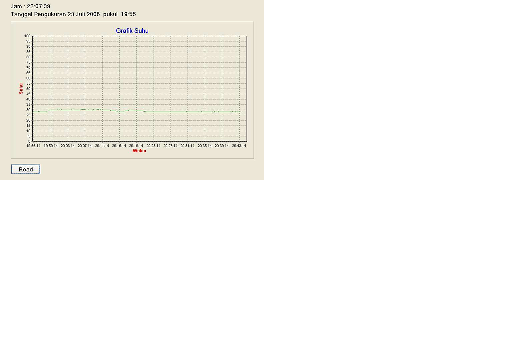
\includegraphics{gambar/3}
    \caption{Tampilan Besar Suhu Terhadap Waktu }
    \label{kripto}
\end{figure}





%-----------------------------------------------------------------
%Disini akhir masukan Bab
%-----------------------------------------------------------------

%-----------------------------------------------------------------
%Disini awal masukan untuk Daftar Pustaka
%-----------------------------------------------------------------
%%\nocite{Abel2010,Guerbas201350}
%%\bibliography{research-plan}
%%\bibliographystyle{plainnat}
\begin{thebibliography}{9}

\bibitem[lima(2013)]{lima05}
Oetomo, Budi Sutedjo Dharma. (2004 \emph{Kamus ++ Jaringan Komputer, edisi
ke-3.}.

\bibitem[dua(2003)]{dua02}
Tanenbaum, Andrew . (2003). \emph{Computer Networks, fourth edition. Prentice Hall, New Jersey.}.

\bibitem[tiga(2004)]{tiga03}
Stallings, William. (2004). \emph{Komunikasi Data dan Komputer Jaringan Komputer. Elex Media, Jakarta.
}.

\bibitem[empat(2013)]{empat04}
Akin, D., Jones, J., Turner, S. (2002). \emph{Certified Wireless Network Administrator Official Study Guide. Planet3 Wireless, Inc., Bremen.}. 
 


\end{thebibliography}
\addcontentsline{toc}{chapter}{DAFTAR PUSTAKA}
%-----------------------------------------------------------------
%Disini akhir masukan Daftar Pustaka
%-----------------------------------------------------------------

\end{document}
